
Figura xx mostra micrografia de um espécime como temperado, sendo observa uma dispersão homogênea de nódulos de grafita. A fração volumétrica de grafita foi determinada por quantificação estereológico como $10.3 \pm 0.5$~\%vol. Na Figura xx a microstrutura atacada do material temperado mostra que a matriz apresenta martensita em morfologia de placas, típica de ligas de alto carbono. A distribuição do tamanho das placas é heterogênea, sendo as maiores placas tão grandes quanto \SI{30}{\micro\meter} e menores placas observadas entre as maiores. As maiores placas de martensita foram as primeiras a se formarem quando a temperatura Ms é atingida durante o resfriamento. As placas menores se formaram sob super-resfriamentos maiores preenchendo as regiões de austenita não-transformada entre as placas de martensita pré-existentes.

\begin{figure*}
  \centering
  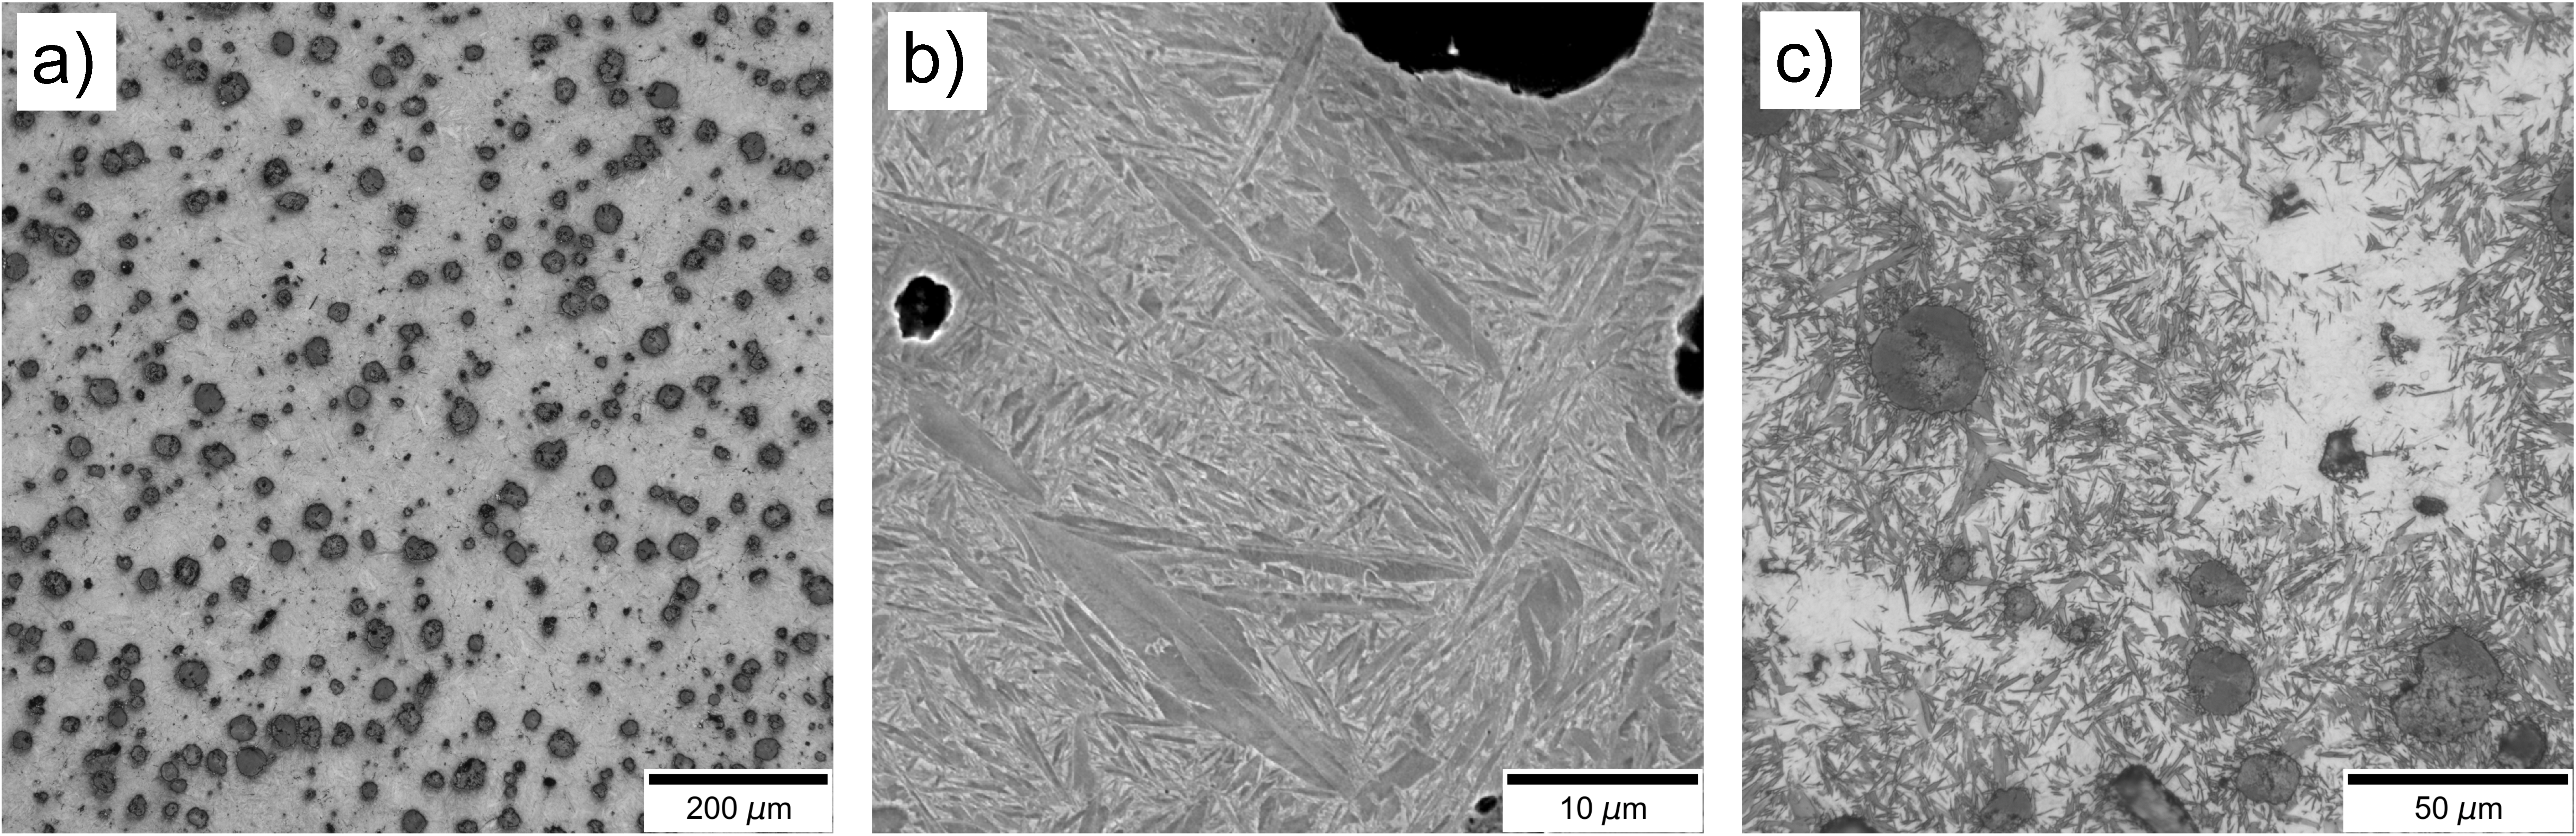
\includegraphics[width=.8\textwidth]{img/martensite.pdf}
  \caption{a) Optical and b) SEM micrographs of the as-quenched specimen. c) Optical micrograph of the sample quenched at 170~°C for 1~min and cooled to room temperature.}
  \label{fig:tempera}
\end{figure*}

A microestrutura da amostra temperada a 170~°C por 1~min e então resfriada até a temperatura ambiente é mostrada na Figura xx. As placas de martensita com aspecto escurecido devido ao ataque metalográfico revela que a estrutura da martensita antes da etapa de partição. Regiões claras correspondem ao agregado de austenita retida e martensita fresca formada durante o resfriamento final. Este microconstituinte é comumente referido na literatura como MA. A martensita formada durante a primeira etapa de têmpera a a 170~°C ($\approx$~43~\%vol.) é ligeiramente revenida durante a etapa isotérmica na etapa de têmpera. Consequentemente esta martensita se comporta diferentemente da martensita presente no microconstituinte MA durante o ataque pelo reagente Nital. É observado que a distribuição da martensita primária é heterogênea. Regiões próximas a nódulos de grafita apresentam maior fração de martensita revenida, enquanto regiões distantes dos nódulos quase não apresentam martensita. Este comportamento é explicado por mudanças locais na temperatura Ms devido à microssegregação formada durante a solidificação.

A microssegregação foi quantificada por Análise de Microssonda Eletrônica (EPMA) em uma amostra temperada a 170~°C e particionada a 375~°C por 15~min. Figuras \ref{fig:EPMA}a--c mostram os mapas de composição dos elementos Si, Mn e Cu, respectivamente. Uma vez que a temperatura de partição é relativamente baixa e o tempo curto, a redistribuição dos elementos substitucionais é desprezível nas etapas posteriores à austenitização. Dessa forma, a distribuição de elementos de liga na condição de análise deve ser compatível com a condição temperada e os demais tratamentos T\&P. Tons de cores representam a porcentagem em peso de cada elemento, como indicada pela escala de cor na parte inferior de cada figura. Nos mapas, a grafita é identificada como regiões em azul, uma vez que a grafita possui virtualmente solubilidade zero destes elementos. Regiões próximas aos nódulos de grafita apresentam maiores teores de Si e Cu, enquanto o Mn segrega para regiões de contornos de célula eutética, as últimas regiões a se solidificar. Este comportamento pode ser melhor visualizada no perfil de composições em linha mostrado na Figura \ref{fig:EPMA}d. Considerando apenas a região da matriz do material, a composição de Si varia entre 1.72--2.89~\% e o Mn varia entre 0.19--0.38~\%. O comportamento da microssegregação destes elementos no ferro fundido é associado às diferentes solubilidades de cada elemento nas fases líquida e sólida (austenita) durante a solidificação e é prevista por simulações Scheil.

\begin{figure}
  \centering
  \includegraphics[width=.9\textwidth]{img/EPMA.pdf}
  \caption{Composition distribution of substitutional elements measured by EPMA. a) Si, b) Mn, c) Cu. d) Composition profiles measured along the probe line drawn over composition maps. e) Predicted local martensite phase fraction ($f^{\alpha'}$) after quenching at 170~°C. f) Histogram showing distribution of $f^{\alpha'}$ after quenching at 170~°C and 25~°C (room temperature).}
  \label{fig:EPMA}
\end{figure}

A distribuição de carbono não foi medida diretamente por EPMA, mas foi determinada utilizando cálculos termodinâmicos e é mostrada no perfil de composição na Figura \ref{fig:EPMA}d. Devido à alta mobilidade do carbono é razoável assumir que após a austenitização a 880~°C o potencial químico do carbono (ou atividade do carbono) é homogêneo ao longo da austenita. Sob essa consideração, o potencial químico do carbono $\mu_C$ para a composição média da liga foi determinado utilizando cálculos termodinâmicos. Usando o valor de $\mu_C$ e o conjunto de composições de Si, Mn e Cu determinados por EPMA cálculos termodinâmicos foram conduzidos de forma a determinar a concentração local de carbono. Como mostrado na Figura \ref{fig:EPMA}d, assim como ocorre com o Mn, o carbono apresenta maior concentração próximo aos contornos de célula (0,87~\%) do que nas proximidades dos nódulos de grafita (0,71~\%).

Tendo a descrição completa das composições de C, Mn, Si e Cu no material após a austenitização, a variação da temperatura Ms de acordo com as variações de composição foram determinadas utilizando a seguinte equação empírica para a temperatura Ms \cite{VanBohemen2012}:

\begin{align}
  Ms\,\text{(°C)} &= 565 - 600 \left[1 - \exp \left( -0.96 w_C^\gamma \right)\right] - 31 w_{Mn}^\gamma \nonumber\\
                & - 13 w_{Si}^\gamma
  \label{eq:MsVanBohemen}
\end{align}
%
em que $w^j_\gamma$ é a porcentagem em passa do elemento $j$ dissolvido na austenita. A temperatura Ms calculada para a composição média da austenita é 215~°C, abaixo da temperatura Ms experimental determinada por dilatometria, mas que está de acordo com a temperatura Ms' da equação de Kostinen-Marburger. Subsequentemente, a temperatura Ms calculada para cada conjunto de composições foi substituída no lugar do parâmetro Ms' na equação \ref{eq:KM}. As equações modificadas foram então utilizada para estimar a fração local de martensita a uma determinada temperatura de têmpera. Figuras xxa--c mostram as distribuições de martensita esperadas após têmpera a 140, 170 e 200~°C, respectivamente. Para têmpera a 170~°C a fração de martensita em contornos de célula eutética é prevista para ser próxima de zero, de acordo com as observações microestruturais mostradas na Figura \ref{fig:tempera}c. Histogramas mostrados na Figura xxd descrevem as distribuições estatísticas de martensita na matriz do ferro fundido temperado a 25, 140, 170 e 200~°C. A fração média de martensita --- representada pelas linhas tracejadas verticais --- estão de acordo com os valores previstos pela aplicação da equação de Kostinen-Marburger (eq. \ref{eq:KM}). Percebe-se que as distribuições são mais largas quanto maior a temperatura de têmpera. Isto significa que temperaturas mais baixas de têmpera levam a uma distribuição mais homogênea de martensita na matriz do material, parcialmente diminuindo os efeitos da microssegregação de elementos.